\documentclass{article} % For LaTeX2e
\usepackage{nips13submit_e,times}
\usepackage[colorlinks=true, urlcolor=blue]{hyperref}
\usepackage{url}
\usepackage{graphicx}
\usepackage{amssymb}
\usepackage{amsmath}


\title{Popularity of content leads to its duplication on Reddit}

\author{
Suren Nihalani \\
\And
Revant Kumar \\
\And
Ashwini Khare \\
\And
Prajwal Prasad
}

% The \author macro works with any number of authors. There are two commands
% used to separate the names and addresses of multiple authors: \And and \AND.
%
% Using \And between authors leaves it to \LaTeX{} to determine where to break
% the lines. Using \AND forces a linebreak at that point. So, if \LaTeX{}
% puts 3 of 4 authors names on the first line, and the last on the second
% line, try using \AND instead of \And before the third author name.

\newcommand{\fix}{\marginpar{FIX}}
\newcommand{\new}{\marginpar{NEW}}

\nipsfinalcopy % Uncomment for camera-ready version

\begin{document}

\maketitle

\begin{abstract}
On social network sites like Reddit, users submit links or share textual content. The community upvotes (for) and downvotes (against) and reddit uses community sourcing as a means to order content. The contributed are scored that is number of upvotes minus downvotes. The popularity of a user is represented by his/her karma. In this project, we have tried to judge how the popularity of contents leads to its duplication on Reddit. Users can re-post the popular posts on various other subreddits in order to receive more upvotes, and thus increasing their karma. Here, we are looking users in two ways, one being the initial person broadcasting the link trying to obtain the critical mass and second one being people reposting content. The results from this project will depict how the users satisfy their Reddit Karma and the design implications of this in online communities. 
\end{abstract}

\section{Objectives}
In this project, we have looked at the following interesting phenomenon:

\begin{equation} 
Karma\ in\ one\ reddit\ \ \ \ \propto\ \ \ \ repost  \nonumber
\end{equation}

Thus, we have mainly focusing on to depict how the users satisfy their Reddit Karma and the design implications of this in online communities. We have correlated a post's score with its diffusion into other subreddits. We have tried to answer the questions such as -- How often do links get reposted?, How many times does a user try to broadcast a link initially? We are trying to see whether there is a relationship between karma and repost frequency.


\section{Background Study}

As social networks and the user-generated content that populates them continue to grow in prevalence, size, and influence, understanding how users interact and produce this content becomes increasingly important. Insight into these community dynamics could prove valuable for measuring content trust, providing role-based group recommendations, or evaluating group stability and growth. For the related work, we have done readings of three papers, namely, Eric Gilbert's - ``Widespread Under Provision on reddit'', Cody Buntain's - ``Identifying social roles in reddit using network structure'' and Donn Morrison's - ``Here, have an upvote: communication behavior and karma on Reddit''.

Online communities rely on their members to do work for the good of everyone on the site. The links with the most up-votes bubble up to the main page, pointing everyone toward the best content. However, when too many people rely on others to contribute without doing so themselves results in under-provision. Gilbert observed that Reddit overlooked 52\% of the most popular links the first time they were submitted [1]. This suggests that many potentially popular links get ignored, thus jeopardizing the site's core purpose of showing the best voted content. 

%Cody Buntain has identified well-known behavioral patterns and social roles in the multi-community environments. In his paper, he has demonstrated the presence and identifiability of the answer-person role in reddit and showed that only a very small number of users participate across community boundaries [2]. 
				
%Donn Morrison has tried to cluster the users of Reddit.com into behavioural roles using features derived from their egocentric reply-graphs. He has tried to explore the link between the distribution of karma (i.e. popularity measured by the number of up- and downvotes) and the behavioural role to which that user belongs. He observed that users with Contributor behaviour proved to be more popular, however the variance in karma in this role was high [3]. Thus, this indicates that the contributor role encompasses both popular and unpopular users. By predicting high-karma users, community owners or moderators, or even the users themselves, could more efficiently manage and maintain behaviour in the forums such as Reddit.com under analysis.	

The other two mentioned papers have tried to examine the users and the data posted by them on Reddit.com. They demonstrated that most of the popular links are overlooked in the first time, only a small number of users participate across community boundaries and the behavioral role of the user is directly linked to the distribution of karma. 

In this project, we are also trying to examine the users and their activity. We are trying to demonstrate that popularity of content leads to its duplication on Reddit. In order to achieve this, we have used the Reddit API to collect the data across various subreddits at various times of the day. 

Some of the questions that we have tried to answer in our project are as follows:

\begin{itemize}
\item How often does reposting of content happen?
\item Is there a triggering score at which reposts occur? 
\item Which subreddits are the first places of the posting? 
\item Is it that less common subreddits get content first because it's easier to reach the front page? 
\item How often do links do well in one subreddit and in other ones? 
\end{itemize}

\section{Data Collection}

We split the data collection into two phases. 

During the first phase, we choose 12 subreddits to monitor. Thanks to \href{http://redditlist.com/}{http://redditlist.com/} we were able to look at sub reddits ordered by highest subscribers. The subreddits chosen for this study were: 

\begin{itemize}
\item /funny
\item /adviceanimals
\item /videos
\item /music
\item /technology
\item /nottheonion
\item /punny
\item /adviceatheists
\item /youtube
\item /radioreddit
\item /programming
\item /theonion
\end{itemize}

Reddit has two types of submissions, namely links and self posts. Self posts are textual submissions. We decided to only look at links because links are binary in the sense that either link leads to the same content or it doesn't. Textual posts might have similar meaning but text might be different. For the purposes of this study, we are only looking at links. 

Every minute, for 8 days, we took a snapshot of all links shared in /new and /hot queue of these subreddits. After 8 day, we wait for five days hoping that most diffusion of links has occurred by then. Our assumption here is that people will share links that they will see links only on the popular page and by five days, the popularity would have been flushed well. 

Now, in the second phase, we take each of the links, and see what other subreddits it has been posted in. We store the map of link to posts in other subreddits. This comprises our data set. 

For the period of 8 days, we managed to get hold of about 42992 posts. Out of these posts, there were about 33044 unique authors and there were about 7541 posts with at-least one repost.

\iffalse
\subsection{Identification of Subreddits}

So far, We chose subreddits related to photography. This was done as all reddit posts on such subreddits use image sharing services like imgur.com. These sharing services usually generate an unique url for each gallery that can be used to share on reddit. Hence, by searching for posts with same image urls, we were able to identify duplicate posts.

Reddit has an inbuilt subreddit recommendation system which lists down relevant subreddits for every search query. These subreddits have a varying frequency of user posts, thus giving a uniform result instead of results being biased to only few with the maximum activity. We choose 10 subreddits to get a preliminary idea about the posts and users in a subreddit.

The subreddits chosen for this study were: 

\begin{itemize}
\item /funny
\item /adviceanimals
\item /videos
\item /music
\item /technology
\item /nottheonion
\item /punny
\item /adviceatheists
\item /youtube
\item /radioreddit
\item /programming
\item /theonion
\end{itemize}

For the project rest of the semester, we plan to re-choose subreddits after a meeting with the professor. Since search allows us to search throughout reddit, we don't have to pick subreddits close to each other. 

\subsection{Fetching and Storing}

We then used Reddit API to retrieve the content (link submissions on hot page) from these subreddits by using an API wrapper (PRAW - python reddit api wrapper) provided for Python language. The script was executed for one hour each on four different times in the same day, to add the dimension of time in our content analysis. A MySQL database was used to store and update the tables of the content which was fetched. While data collection of top and news posts is running, in parallel, we also run a bot that looks at posts that has been collected more than 5 days in the past and we look up where have these links diffused in reddit and stores the tuple (link, sub\_reddit, poster, time\_created) into the db. 
\fi

\section{Data Analysis}

The statistics of the data collected can be seen in Table1.

\begin{table}
\begin{center}
    \begin{tabular}{ | l | l | }
    \hline
    Number of Posts & 42992 \\ \hline
    Number of Unique Authors & 33044 \\ \hline
    Number of links reposted at least once & 7541 \\ \hline
    \end{tabular}
    \caption{Data Analysis}
\end{center}
\end{table}

\subsection{Chains}

Once we have obtained all the posts, we search each of the posts on reddit in order to get their diffusion across the various sub-reddits since their inception. Thus, we thinking of the search results like a diffusion chain. We have sorted the results by time and we call the first person to post the link as the original author. How many times the original author posts initially is how much effort he puts into broadcasting the link. After this, we have found the search result with max score so that we can know when a particular reached its maximum popularity. All results to the left of the max post form the left chain and after wards form the right chain.

An example of chains can be seen in the following figure:

\begin{figure}[h]
\begin{center}
%\framebox[4.0in]{$\;$}
%\fbox{\rule[-.5cm]{0cm}{4cm} \rule[-.5cm]{4cm}{0cm}}
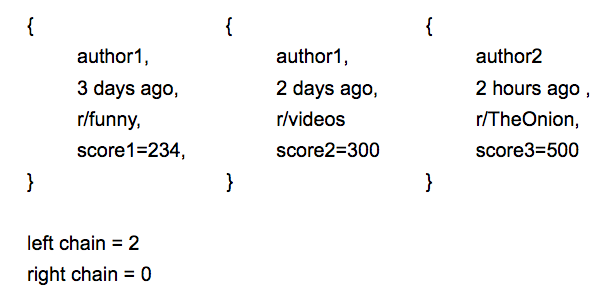
\includegraphics[width=5in]{chain.png}
\caption{Description of Chain}
\end{center}
\end{figure}

In this example, we have three results, the last result has the max score, so our left chain length is 2 and right chain length is 0.  Note that we don?t do normalization with respect to how many subscribers are in the subreddit.



\subsection{Distribution of Chain Length}

Figure 2 shows distribution of chain length of posts i.e. distribution of how far links go. It can be observed that most chain lengths are less than 50. There is a decreasing trend in distribution. Thus, posts with longer chains are less in number. However, there is one anomaly. We notice a tiny growth at the end near the 230-240 bucket with like nothing in between. This post has 235 shares and turned out to be a spam link where every-time a randomly generated unique author posted in /r/funny.

The average chain length was found to be 1.68 with a standard deviation of 2.88.

\begin{figure}[h]
\begin{center}
%\framebox[4.0in]{$\;$}
%\fbox{\rule[-.5cm]{0cm}{4cm} \rule[-.5cm]{4cm}{0cm}}
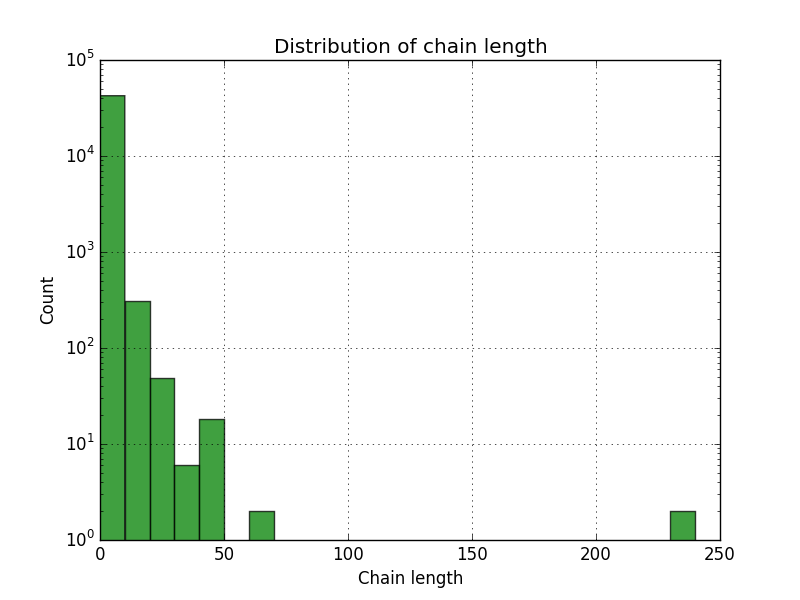
\includegraphics[width=4.0in]{lengths.png}
\caption{Distribution of Chain Length}
\end{center}
\end{figure}


\subsection{Distribution of Original Author Re-posting}

Figure 3 shows that distribution of posts by the original author. So, it basically shows the the number of times the original author is reposting his/her own link in order to broadcast it so that it becomes more popular which eventually leads to a higher karma for him/her. We observed that the maximum number of times author has reposted has gone to 12 in our dataset.

The original author makes a submission more than once  ~7\% of the times. When we considered only posts that had been reposted at least once, we found that in around 28.8\% of the cases, the original author had made a submission more than once. 

\begin{figure}[h]
\begin{center}
%\framebox[4.0in]{$\;$}
%\fbox{\rule[-.5cm]{0cm}{4cm} \rule[-.5cm]{4cm}{0cm}}
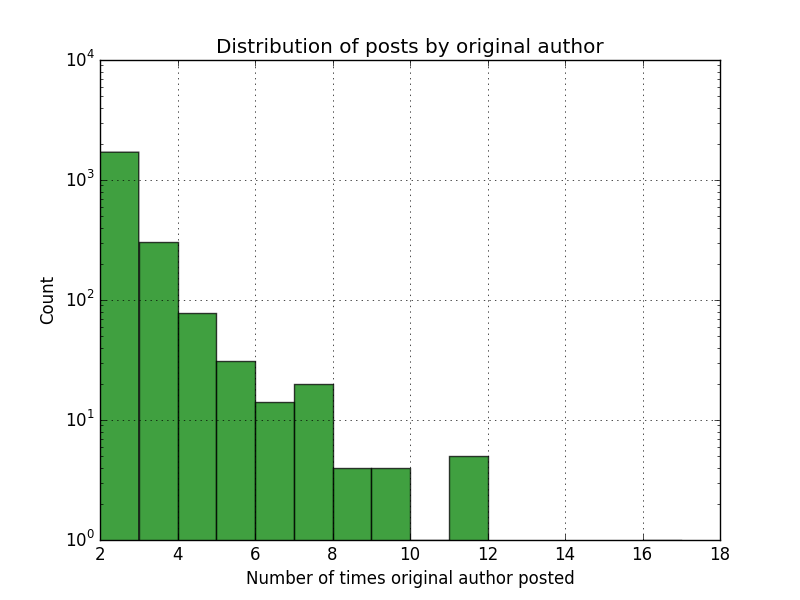
\includegraphics[width=4.0in]{original_author.png}
\caption{Distribution of Original Author Re-posting}
\end{center}
\end{figure}

\newpage

\subsection{Distribution of Re-posts by each Subreddit}

Figure 4 shows the distribution of posts and re-posts by each subreddit. Thus, here we are looking how much repost happens in each subreddit. We were expecting a lot of reposts from subreddits adviceanimals or funny because most of them are meme based subreddits but programming and technology came out on the top. 
It is interesting to note that ~73\% of the posts in subreddit technology were reposts. 

\begin{figure}[h]
\begin{center}
%\framebox[4.0in]{$\;$}
%\fbox{\rule[-.5cm]{0cm}{4cm} \rule[-.5cm]{4cm}{0cm}}
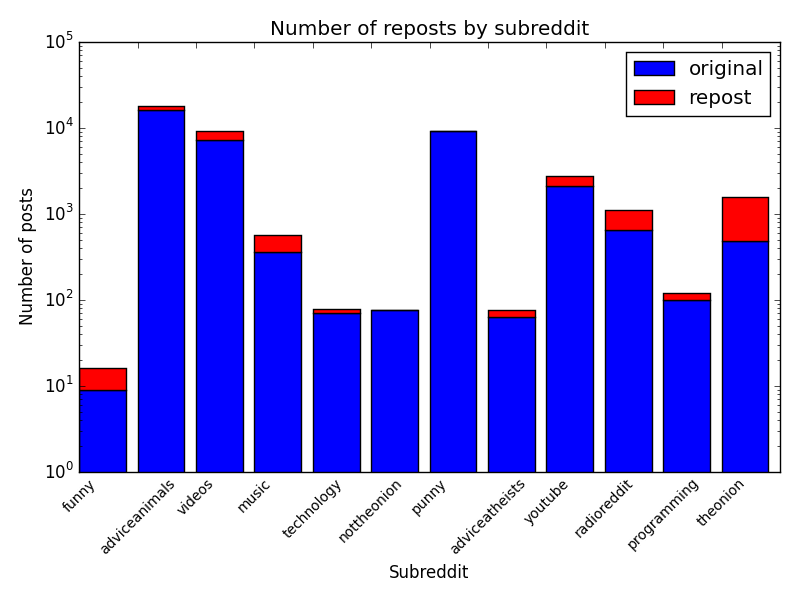
\includegraphics[width=3.5in]{reposts.png}
\caption{Distribution of Re-posts by each Subreddit}
\end{center}
\end{figure}


\subsection{Distribution of Different Authors Re-posting}

Figure 5 shows the distribution of different authors re-posting. So basically it calculates a ratio of unique authors by the chain length. If this ratio is 1, this means that all authors in post's chain are unique. We observed that that ratio is 1 in most of the cases. Thus, the chain of most of the posts on Reddit consist of unique authors i.e. most of the time it's only unique people who are reposting. 
We observe that around  77.36\% of times, the reposts by different authors is more than those by the same author.

\begin{figure}[h]
\begin{center}
%\framebox[4.0in]{$\;$}
%\fbox{\rule[-.5cm]{0cm}{4cm} \rule[-.5cm]{4cm}{0cm}}
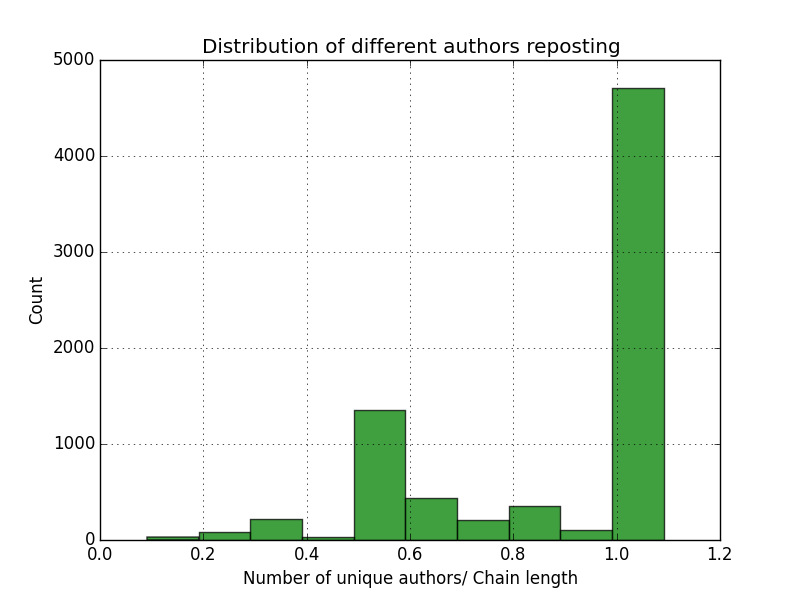
\includegraphics[width=3.5in]{unique_authors.png}
\caption{Distribution of Different Authors Re-posting}
\end{center}
\end{figure}

\newpage

\subsection{Distribution of Left Chain Length}

Figure 6 shows distribution of left chain length. This distribution basically shows us how people try to make a particular post happening and popular. It tells the factors that led to the post's maximum popularity in the entire chain. It is observed that left chain for most posts is less than 30. Also, a decreasing behavior is observed as expected. However, again there is an anomaly in the graph near the 225-230 bucket. We looked at it, that post has a left chain length of 229 and found that it turned out to be a spam link where every-time a randomly generated unique author posted in /r/funny.
The average left chain length was found to be 0.231 with a standard deviation of 2.015.

\begin{figure}[h]
\begin{center}
%\framebox[4.0in]{$\;$}
%\fbox{\rule[-.5cm]{0cm}{4cm} \rule[-.5cm]{4cm}{0cm}}
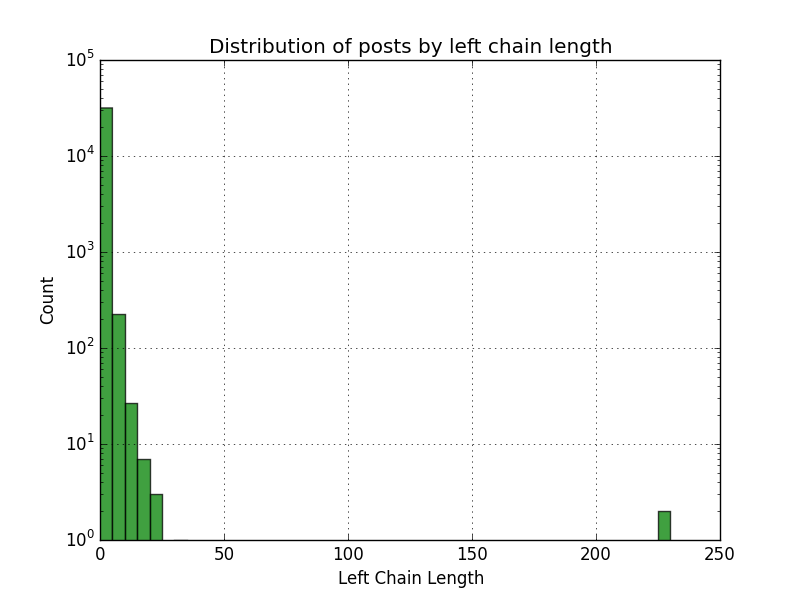
\includegraphics[width=3.5in]{left_chain.png}
\caption{Distribution of Left Chain Length}
\end{center}
\end{figure}

\subsection{Distribution of Right Chain Length}

Figure 7 shows the distribution of the right chain length. It basically shows how far diffusion of a link can go. It was observed that no link made it more than 50 reposts after the point in the chain when the post was at its highest popularity. Also, a decreasing behavior was observed. 
The average right chain length was found to be 0.45 with a standard deviation of 1.76.

\begin{figure}[h]
\begin{center}
%\framebox[4.0in]{$\;$}
%\fbox{\rule[-.5cm]{0cm}{4cm} \rule[-.5cm]{4cm}{0cm}}
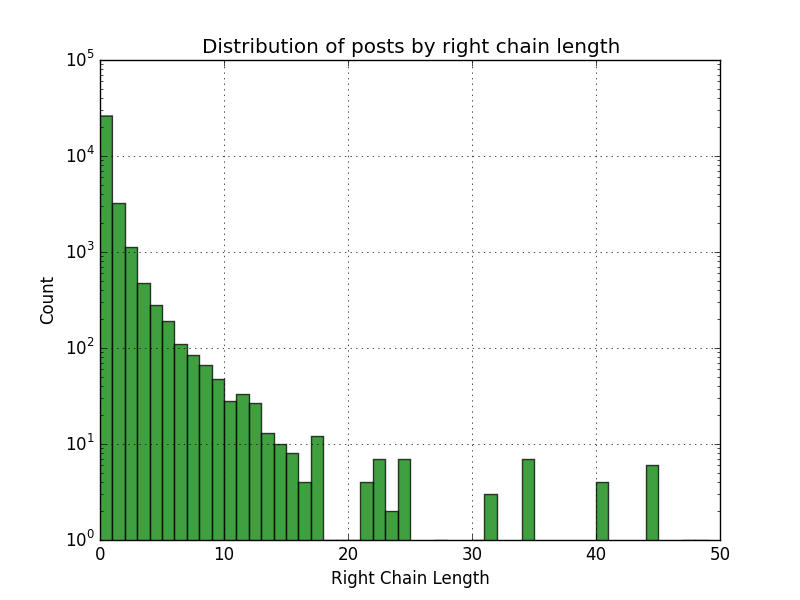
\includegraphics[width=3.5in]{right_chain.png}
\caption{Distribution of Right Chain Length}
\end{center}
\end{figure}

\newpage

\subsection{Distribution of Max Score by the Right Chain Length}

Figure 8 shows the scatter plot of the maximum score achieved and the right chain length of each post in the data-set. So, it was observed that for most of the posts, the right chain length is less than 20 even for very high maximum scores. Also, some unexpected results were observed such that some posts with even very low maximum score had very large right chain length and some posts with very high maximum score has very small right chain length.
The pearson correlation coefficient between between max score and right chain length is 0.24 which suggests that there is some correlation between the two, but it is of a lower degree.

\begin{figure}[h]
\begin{center}
%\framebox[4.0in]{$\;$}
%\fbox{\rule[-.5cm]{0cm}{4cm} \rule[-.5cm]{4cm}{0cm}}
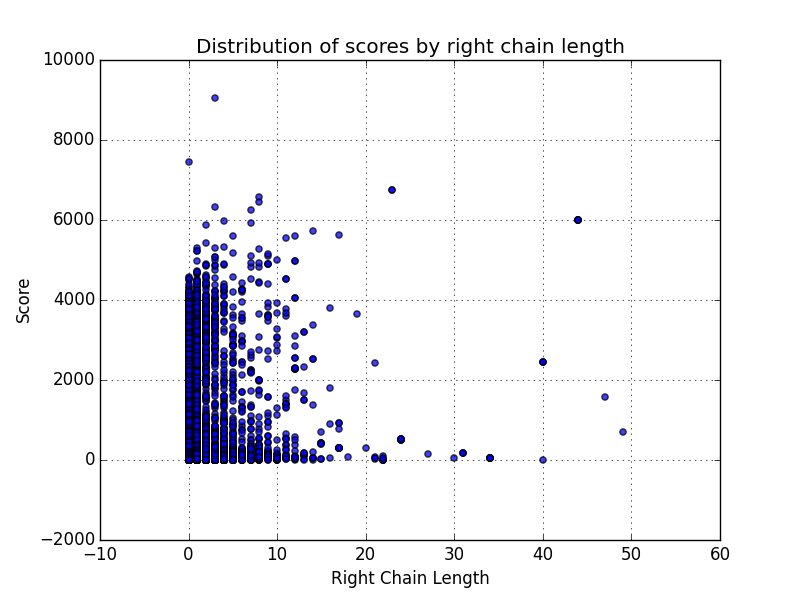
\includegraphics[width=3.6in]{score_right_chain.png}
\caption{Distribution of Max Score by the Right Chain Length}
\end{center}
\end{figure}

\subsection{Distribution of Maximum Score of the chains}

Figure 9 shows the distribution of the maximum score of the chains in our dataset. We had expected the figure to be at highest around the low scores, and have a decreasing nature with a long tail. However, we noticed a surge in posts with scores around 3000.

\begin{figure}[h]
\begin{center}
%\framebox[4.0in]{$\;$}
%\fbox{\rule[-.5cm]{0cm}{4cm} \rule[-.5cm]{4cm}{0cm}}
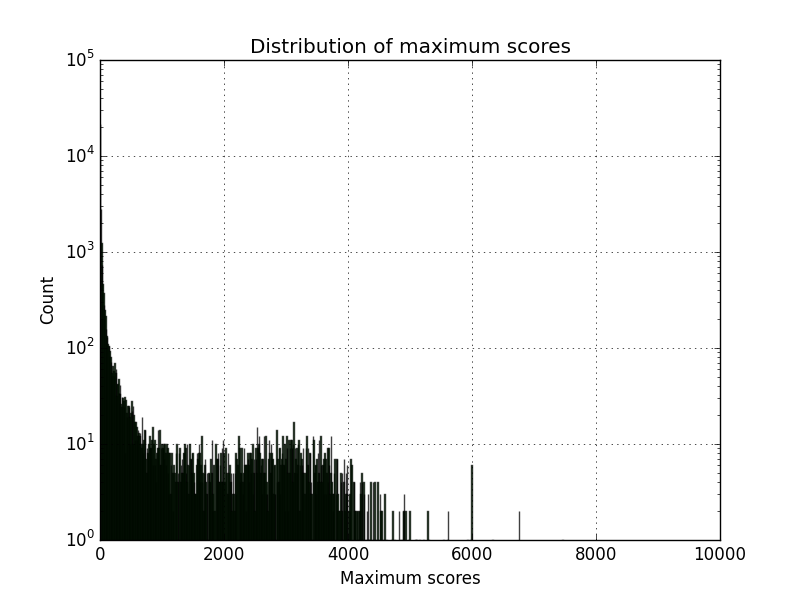
\includegraphics[width=3.6in]{max_score_distribution.png}
\caption{Distribution of Maximum Score of the chains}
\end{center}
\end{figure}

\newpage


\section{Comparison with Eric Gilbert's Paper on Widespread Under-provision on Reddit}

We compared our results with a related study done by Eric Gilbert who found that only around half of the popular links were noticed in the initial submission. Gilbert?s dataset was popular links from /r/pics subreddit. We found similar results when we evaluated the same figures for our dataset of 12 sub-reddits.

\begin{itemize}
\item Widespread Under Provision on reddit -- Eric Gilbert
	\begin{itemize}
	\item Analyzed 9,370 popular links
	\item 48\% links noticed on first submission
	\item Refer figure 12
	\end{itemize}
	
	\begin{figure}[h]
	\begin{center}
	%\framebox[4.0in]{$\;$}
	%\fbox{\rule[-.5cm]{0cm}{4cm} \rule[-.5cm]{4cm}{0cm}}
	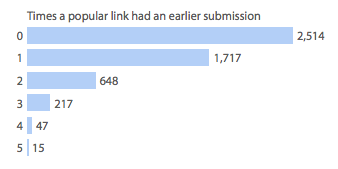
\includegraphics[width=3.8in]{eric.png}
	\caption{Times a popular link has an earlier submission}
	\end{center}
	\end{figure}
	
\item Our Study
	\begin{itemize}
	\item Analyzed 42,992 links
	\item 12 subreddits
	\item 78.28\% links noticed on first submission
	\item Refer figure 13
	\end{itemize}
	
	\begin{figure}[h]
	\begin{center}
	%\framebox[4.0in]{$\;$}
	%\fbox{\rule[-.5cm]{0cm}{4cm} \rule[-.5cm]{4cm}{0cm}}
	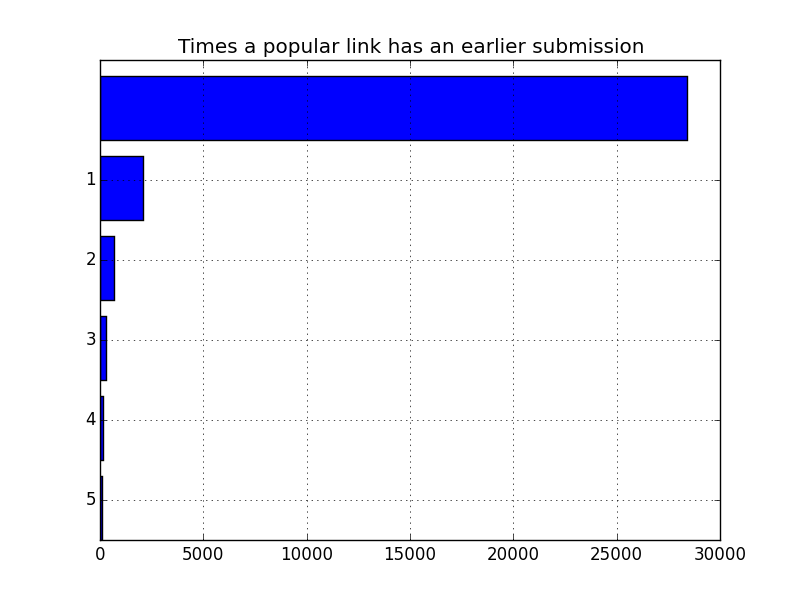
\includegraphics[width=3.7in]{count.png}
	\caption{Times a popular link has an earlier submission}
	\end{center}
	\end{figure}
\end{itemize}

\newpage


\section{Anomalies with the Data}

\subsection{Forbidden Links}

We found some posts that reddit has banned directly on API level. An online search of the given link redirected to a 403 Forbidden Error page. Interestingly, the link has a politically sensitive article. Moreover, it is no where mentioned in their API documentation to get an error of this nature. One of such pages can be seen in the following image:

\begin{figure}[h]
\begin{center}
%\framebox[4.0in]{$\;$}
%\fbox{\rule[-.5cm]{0cm}{4cm} \rule[-.5cm]{4cm}{0cm}}
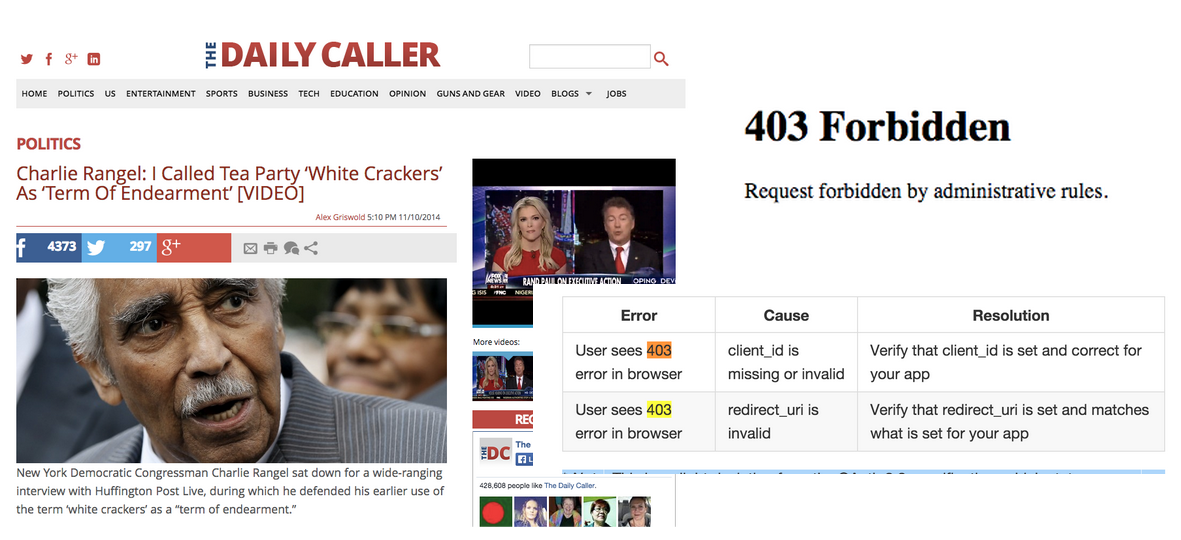
\includegraphics[width=4.6in]{pol.png}
\caption{Link which is forbidden on Reddit}
\end{center}
\end{figure}

\subsection{Posts having chain length of 235}

Post having a chain length of 235 was too good to be true. So, we checked it manually and found that it turned out to be a spam link where every-time a randomly generated unique author posted in /r/funny. It's pretty creepy to see that someone is using the API to growth hack their website.  The domain name is expired. It doesn't make sense. A screenshot of that page is shown below:

\begin{figure}[h]
\begin{center}
%\framebox[4.0in]{$\;$}
%\fbox{\rule[-.5cm]{0cm}{4cm} \rule[-.5cm]{4cm}{0cm}}
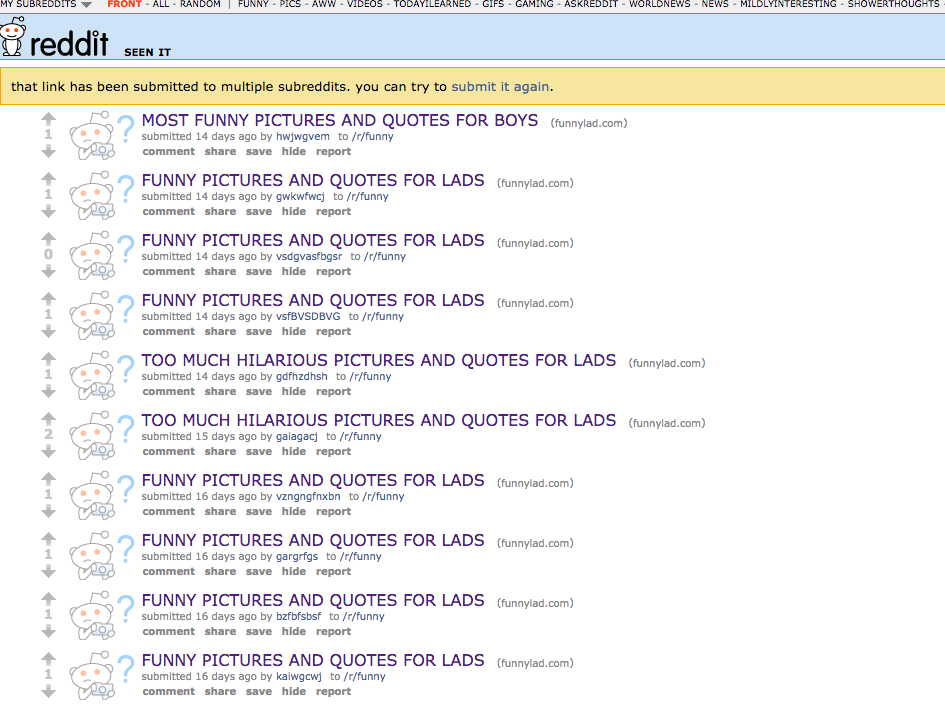
\includegraphics[width=4.5in]{funny.png}
\caption{Post with a chain length of 235}
\end{center}
\end{figure}

\newpage

\subsection{Exception Handling and Issues with PRAW}

We just wanted to point out the difficulties that we faced in data collection. A lot of exception handling had to be done to take care of various issues to collect a dataset with a decent number of records. We had email alerts set up to notify whenever our bot found a new error. Also, the python wrapper we used to collect data had its own issues which forced us to recollect data in Phase 2.

\section{Conclusion and Future Work}
In this project, we make a number of interesting observations and obtain some useful insights on content duplication in reddit. We observe that in some subreddits such as r/technology, around 73\% of the links have already been submitted before. We find that ~22\% of the posts have gained more scores(upvotes-downvotes) when they have been resubmitted. Also, we find that the chain length after a post gains popularity is around twice the chain length before a post has reached its maximum score in the chain. Although the extent of correlation isn't great, we find that correlation exists between a post's top score and the post being reposted, which suggests that popularity may be a factor in the duplication of content. However, there are some limitations. Firstly, our analysis is limited to the 12 subreddits we have considered. Though we have used both popular and smaller subreddits, the representativeness of the set to be extended to reddit in general needs to be verified. Secondly, we are limited by the reddit API to obtain any information regarding a user's list of subscribed subreddits and his likes or upvotes. Thus it becomes difficult to discern if a user reposted a link after viewing it in a subreddit, or any other source, and whether the post's score influenced him to repost the link. 

One of the research questions that interests us is 'What type of users often make duplicate submissions?' Thus our future work involves studying users reposting behaviour. It would be interesting to find what \% of a user's karma is obtained purely by reposted links. Also, studying a user's reposting behaviour may help us detect spam attempts similar  to the one we detected in this project. 


\iffalse
\section{Work Ahead}
For the second part of the term, we plan to collect data for 15 days from subreddits in different areas of interest and of smaller size with the new and top queue. We are planning to look at the following subreddits as shown in Table 1:

\begin{table}
\begin{center}
    \begin{tabular}{ | l | l | }
    \hline
    Famous Subreddits & Similar smaller subreddits \\ \hline
    funny (6,988,603) & punny (54,491) \\ \hline
    AdviceAnimals (4,252,660) & AdviceAtheists (13,460) \\ \hline
    videos (6,192,963) & YouTube (21,611) \\ \hline
    Music (5,526,808) & RadioReddit (13,356) \\ \hline
    technology (5,066,423) & programming (559,631) \\ \hline
    nottheonion (1,435,635) & TheOnion (6,610) \\ 
    \hline
    \end{tabular}
    \caption{Subreddits we plan to monitor and number of subscribers}
    \end{center}
\end{table}


Thanks to http://redditlist.com/ we were able to look at sub reddits ordered by highest subscribers. The rationale for choosing these subreddits is now changed to be orthogonal in terms of topic of the subreddit because we discovered that we no longer have to do search ourselves and reddit offers searching in all the subreddits with it's API. We wanted to see if there is a trend across different types of content. Reddit has two types of submissions, namely links and self posts. Self posts are textual submissions. We decided to only look at links because links are binary in the sense that either link leads to the same content or it doesn't. Textual posts might have similar meaning but text might be different. For the purposes of this study, we are only looking at links. 

While we'll collect the hot and new stories for each subreddit, we will also run a parallel bot that looks at links that were posted more than four days ago and see what subreddits the link got duplicated to. Now there are three possible scenarios for reposting. One is broadcaster where the user is trying to post the same link with multiple topics in multiple subreddits. We will see if the first link's occurrence has happened within relatively short amount of time in different subreddits by the same author. Another use case is cross posting link where the user is part of one community, while browsing that community, he/she comes across the link and shares in another community. We can use the reddit api to figure out where the links came from by sorting the links by time and then seeing if the original poster of the link is part of any of the subreddits the links in the past were posted in. It's highly probably that the user saw it in another subreddit then. The last one being the user came across the link outside reddit. We are considering if we can maybe survey them and hope users respond with right format of response like SMS voting schemes work these days. There also might be cases where the user doesn't know that the link was being duplicated. 

We plan to identify to see how often does reposting of content happen. Is there is a triggering score at which reposts occur? Which subreddits are the first places of the posting? Is it that less common subreddits get content first because it's easier to reach the front page? How often do links do well in one subreddit and in other ones? We'll consider doing a visualization of how the content diverges.
\fi


\section{Contributions}
We have been contributing about equally in this project. However we have distributed responsibilities based upon areas of interest as shown in Table 2.


\begin{table}
\begin{center}
    \begin{tabular}{ | l | l | }
    \hline
    Team member & Contributions \\ \hline
    Ashwini & Data collection \\ \hline
    Prajwal & Data visualization and scripting \\ \hline
    Revant & Data analysis \\ \hline
    Suren & Development of the bot \\ 
    \hline
    \end{tabular}
    \caption{Contributions}
    \end{center}
    \end{table}



\section{References}
\begin{itemize}
\item Eric Gilbert. 2013. Widespread underprovision on Reddit. In Proceedings of the 2013 conference on Computer supported cooperative work (CSCW '13). ACM, New York, NY, USA, 803-808
\item Cody Buntain and Jennifer Golbeck. 2014 Identifying social roles in reddit using network structure. In Proceedings of the companion publication of the 23rd international conference on World wide web companion (WWW Companion '14) International World Wide Web Conferences Steering Committee, Republic and Canton of Geneva, Switzerland, 615-620
\item Morrison, Donn, and Conor Hayes. 2013. Here, have an upvote: communication behaviour and karma on Reddit. GI-Jahrestagung
\end{itemize}

\end{document}
